% ============================================================
% Informe final en formato IEEE (conferencia). Versión LaTeX del
% documento de 05-informe/documento/.
% Compilar desde esta carpeta:
%   pdflatex main.tex
%   bibtex main
%   pdflatex main.tex
%   pdflatex main.tex
% ============================================================
\documentclass[conference,a4paper]{IEEEtran}

\usepackage[utf8]{inputenc}
\usepackage[T1]{fontenc}
\usepackage[spanish,es-tabla]{babel}
\usepackage{amsmath,amssymb}
\usepackage{array}
\usepackage{longtable}
\usepackage{graphicx}
\usepackage{cite}
\usepackage{url}
\usepackage[hidelinks]{hyperref}

\graphicspath{{imagenes/}}

% Rótulos al estilo IEEE: "Resumen", "Palabras clave" y "Fig."
\addto\captionsspanish{%
  \renewcommand{\abstractname}{Resumen}%
  \renewcommand{\refname}{Referencias}%
  \renewcommand{\figurename}{Fig.}%
}
\renewcommand{\IEEEkeywordsname}{Palabras clave}

\newcommand{\mn}{\mathop{\text{mín}}\nolimits}

% Columnas de tabla con ancho fijo
\newcolumntype{L}[1]{>{\raggedright\arraybackslash}p{#1}}
\newcolumntype{C}[1]{>{\centering\arraybackslash}p{#1}}
\newcommand{\tablabase}{\renewcommand{\arraystretch}{1.1}\setlength{\tabcolsep}{2.5pt}}

\begin{document}

% ------------------------------------------------------------
% Título y autores
% ------------------------------------------------------------
\title{Identificación de Cuellos de Botella en una Línea de Producción de Muebles de Madera
mediante Simulación de Eventos Discretos en Python}

\author{
\IEEEauthorblockN{Victor Roa, Francis Valdiviezo, Cael Soto, Jimmy Ontaneda y Alejandro Padilla}
\IEEEauthorblockA{\textit{Simulación $\cdot$ Grupo 10 $\cdot$ Carrera de Computación, FEIRNNR}\\
\textit{Universidad Nacional de Loja, Loja, Ecuador}\\
\small victor.roa@unl.edu.ec, francis.valdiviezo@unl.edu.ec, cael.soto@unl.edu.ec,\\
jimmy.ontaneda@unl.edu.ec, alejandro.padilla@unl.edu.ec}
}

\maketitle

\begin{abstract}
La fabricación de muebles de madera comprende varias etapas cuyos diferentes tiempos de
procesamiento pueden generar acumulaciones y limitar la capacidad de producción. Este
trabajo tuvo como objetivo identificar el cuello de botella de una línea de fabricación de
muebles y evaluar alternativas de mejora mediante simulación de eventos discretos en
Python. Se modelaron cuatro estaciones (corte, lijado, ensamblaje y acabado) utilizando
SimPy y una tasa de llegadas de tres muebles por hora. Se realizaron 30 réplicas de
1\,000 horas por escenario, descartando las primeras 100 horas como periodo de
calentamiento. Los resultados se compararon con el modelo teórico de colas M/M/1 mediante
indicadores de utilización, longitud de cola y tiempo de espera. En el escenario inicial,
el ensamblaje presentó la menor capacidad y una espera media de 45,43 minutos. Al reducir
su tiempo de procesamiento de 15 a 12 y 10 minutos, las esperas disminuyeron un
61,99\,\% y un 78,62\,\%, respectivamente. Además, la capacidad nominal de la línea
aumentó de cuatro a cinco muebles por hora, aunque la producción efectiva se mantuvo
cercana a tres. Los errores porcentuales frente a la teoría no superaron el 4,07\,\%. Se
concluye que mejorar la estación crítica permite reducir la congestión y los tiempos de
espera, aunque una mayor capacidad no necesariamente implica un incremento de la
producción efectiva.
\end{abstract}

\begin{IEEEkeywords}
simulación de eventos discretos, teoría de colas, cuello de botella, línea de producción,
Python.
\end{IEEEkeywords}

% ============================================================
\section{Introducción}
% ============================================================
\IEEEPARstart{L}{os} muebles de madera se fabrican por etapas: primero se cortan las
piezas, después se lijan, luego se ensamblan y al final se les da el acabado
\cite{nouri2019,matrani2026,bambura2020}. Cada etapa tarda un tiempo distinto
\cite{nouri2019,bambura2020}, y si una es más lenta que las demás, los muebles se acumulan
antes de ella mientras las siguientes esperan sin trabajo \cite{matrani2026,velumani2017}. A
esa etapa se le llama cuello de botella, y es la que limita cuántos muebles puede entregar
la fábrica \cite{bambura2020,li2020}. Por eso a las fábricas les interesa saber cuál es y
cómo mejorarla.

Probar cambios directamente en la fábrica para ver si mejoran la producción es caro y puede
obligar a parar el trabajo. Por eso se usan simulaciones en computador: se arma un modelo de
la línea y los cambios se prueban ahí antes de hacerlos de verdad
\cite{negahban2014,mourtzis2020}. Una de las más usadas en fábricas es la simulación de
eventos discretos, que sigue lo que le pasa a cada pieza mientras avanza por las etapas.
Negahban y Smith \cite{negahban2014} revisaron cerca de 300 trabajos que la usan en
manufactura, y Mourtzis \cite{mourtzis2020} explica cómo ha cambiado con el tiempo y cómo
ayuda a probar alternativas antes de aplicarlas.

En la industria del mueble ya se ha usado esta técnica. Nouri y Abdul-Nour \cite{nouri2019}
mejoraron una línea donde se ensamblan y terminan varios tipos de muebles; Mat Rani
\textit{et al.} \cite{matrani2026} estudiaron cuántos trabajadores poner en cada proceso
para que se espere menos; y Bambura \textit{et al.} \cite{bambura2020} encontraron que el
lijado y el ensamblaje eran los cuellos de botella en la fabricación de cajoneras, y vieron
que añadir máquinas mejoraba la producción. En otras líneas de producción, Velumani y Tang
\cite{velumani2017} analizaron los cuellos de botella y las piezas acumuladas en una línea
por lotes, y Li \textit{et al.} \cite{li2020} vieron que añadir capacidad en el cuello de
botella ayuda, aunque cada vez menos.

Además de la simulación existe la teoría de colas, que da fórmulas para calcular cuánto se
usa cada máquina y cuánto esperan las piezas \cite{govil1999}. Estas fórmulas también
muestran que, cuando una máquina está muy ocupada, las esperas crecen rápidamente
\cite{wu2012}, y sirven para revisar si una simulación está bien hecha. En la Tabla
\ref{tab:a1} del Anexo A se resume qué hizo cada uno de estos trabajos y qué aporta a este.

Los trabajos revisados muestran un problema que se repite: como cada etapa tarda un tiempo
distinto \cite{nouri2019,bambura2020}, la línea queda desbalanceada y aparecen cuellos de
botella, piezas acumuladas y entregas más lentas \cite{matrani2026,velumani2017}. Arreglarlo
cambiando cosas directamente en la fábrica es caro y arriesgado, porque se puede invertir en
la etapa equivocada \cite{li2020,negahban2014,mourtzis2020}. Además, varios de estos
estudios usan programas comerciales de pago, como Arena \cite{nouri2019,matrani2026} y Plant
Simulation \cite{bambura2020,li2020}. Por eso se propone un modelo en Python, un lenguaje
gratuito, que permita encontrar el cuello de botella y probar mejoras sin costo, y que se
compare con las fórmulas de teoría de colas para comprobar que sus resultados son confiables
\cite{govil1999,wu2012}.

En este informe se simula en Python una línea de producción de muebles de madera con cuatro
estaciones: corte, lijado, ensamblaje y acabado. Primero se identifica cuál estación limita
la producción; luego se comparan tres escenarios de mejora y se contrastan los resultados con
los valores teóricos de colas \cite{govil1999,wu2012}.

% ============================================================
\section{Objetivos}
% ============================================================
\subsection{Objetivo general}
Simular mediante eventos discretos en Python una línea de producción de muebles y comparar
sus resultados con el modelo de colas M/M/1, para identificar la estación de menor capacidad
(cuello de botella) y evaluar cómo realizar mejoras para aumentar la capacidad máxima de
producción de la línea.

\subsection{Objetivos específicos}
\textit{1) Modelado y validación de la línea base:} simular en Python la línea de cuatro
estaciones y validar sus medidas de desempeño frente al modelo M/M/1.

\textit{2) Cuello de botella y escenarios de mejora:} identificar la estación que genera el
cuello de botella y comparar la línea actual con escenarios de mejora que reducen el tiempo
de ensamblaje, evaluando la utilización, la cola, la espera y la capacidad máxima de la
línea.

% ============================================================
\section{Metodología}
% ============================================================
\subsection{Enfoque}
El enfoque es cuantitativo: el trabajo mide indicadores numéricos (utilización, colas y
esperas) y los compara con valores teóricos mediante el error porcentual.

\subsection{Tipo de estudio}
Es un estudio aplicado, pues usa un modelo en Python para estudiar una línea de producción
de muebles de madera con tiempos supuestos, no medidos en una fábrica real, por lo que no es
un estudio de caso como los de \cite{nouri2019} y \cite{bambura2020}. También es
comparativo, porque compara tres escenarios entre sí y la simulación con la teoría M/M/1.

\subsection{Herramientas y recursos}
La Tabla \ref{tab:recursos} resume los recursos utilizados.

\begin{table}[!t]
\caption{Herramientas y recursos}
\label{tab:recursos}
\centering
\footnotesize
\tablabase
\begin{tabular}{|L{2.7cm}|L{5.4cm}|}
\hline
\textbf{Recurso} & \textbf{Descripción} \\ \hline
Lenguaje de programación & Python 3.13.14 (requiere Python 3.12 o superior). \\ \hline
Bibliotecas & SimPy 4.1.2, NumPy 2.5.4, pandas 3.0.6, Matplotlib 3.11.2. \\ \hline
Software & Entorno virtual .venv; pruebas automáticas con pytest 9.1.1. \\ \hline
Hardware & AMD Ryzen 7 7445HS, 14 GiB de RAM. \\ \hline
Conjunto de datos & No se usan datos reales. Los parámetros (llegadas de 3 muebles/h,
tiempos de 8, 10, 15 y 12 min, 30 réplicas de 1\,000 h, 100 h de calentamiento y semilla
2026) son supuestos guardados en archivos de configuración (sección III-D-4). \\ \hline
Modelos matemáticos & Capacidad y utilización, M/M/1, Ley de Little y error porcentual
(sección III-D-5). \\ \hline
\end{tabular}
\end{table}

\subsection{Procedimiento}

\subsubsection{Identificación y análisis del problema}
Se planteó una línea de fabricación de muebles de madera compuesta por cuatro estaciones en
serie: corte, lijado, ensamblaje y acabado. El problema consiste en identificar la estación
que limita la capacidad de producción y evaluar alternativas para reducir su congestión. Cada
estación dispone de un recurso y una cola independiente, atendida por orden de llegada
(FIFO) y sin límite de capacidad. El modelo supone disponibilidad continua de materiales y
excluye fallas de maquinaria, defectos, traslados y reprocesos.

\begin{center}
{\small\textit{Entrada $\rightarrow$ Corte $\rightarrow$ Lijado $\rightarrow$ Ensamblaje
$\rightarrow$ Acabado $\rightarrow$ Mueble terminado}}
\end{center}

\subsubsection{Revisión de literatura científica}
Se revisaron los trabajos científicos presentados en la sección I. Los estudios sobre
simulación en manufactura \cite{negahban2014,mourtzis2020} y fabricación de muebles
\cite{nouri2019,matrani2026,bambura2020} fundamentaron la selección del método. Las
investigaciones sobre cuellos de botella \cite{velumani2017,li2020} permitieron establecer
los indicadores de evaluación, mientras que los trabajos sobre teoría de colas
\cite{govil1999,wu2012,gross2008} proporcionaron las bases matemáticas para contrastar los
resultados de la simulación.

\subsubsection{Selección de los modelos o métodos}
Se utilizó un modelo de simulación de eventos discretos, estocástico y dinámico. Los cambios
de estado ocurren en eventos específicos, como llegadas, inicios y finalizaciones de
operaciones. Su carácter estocástico se debe a que los tiempos entre llegadas y los tiempos
de servicio siguen distribuciones exponenciales. Para evaluar el comportamiento de las
estaciones se empleó el modelo de colas M/M/1, dado que cada una dispone de un único
recurso. También se aplicaron la Ley de Little y el error porcentual para comprobar la
correspondencia entre los resultados simulados y teóricos \cite{gross2008}.

\subsubsection{Definición de variables y parámetros}
Se definieron las entidades, recursos, eventos, variables de estado e indicadores necesarios
para representar el funcionamiento de la línea de producción. Estos elementos se presentan en
la Tabla \ref{tab:elementos}, mientras que la Tabla \ref{tab:parametros} recoge los
parámetros iniciales de las cuatro estaciones, incluyendo el número de recursos, los tiempos
medios de procesamiento y sus capacidades.

\begin{table}[!t]
\caption{Elementos del modelo de simulación}
\label{tab:elementos}
\centering
\footnotesize
\tablabase
\begin{tabular}{|L{2.3cm}|L{5.8cm}|}
\hline
\textbf{Elemento} & \textbf{Definición operacional} \\ \hline
Entidad & Un mueble que pasa por corte, lijado, ensamblaje y acabado. \\ \hline
Recursos & Operario y equipo de cada estación; cada uno atiende un mueble a la vez. \\ \hline
Colas & Muebles que esperan mientras la estación está ocupada. \\ \hline
Eventos & Llegada, entrada a la cola, inicio y fin de una operación, y salida del mueble
terminado. \\ \hline
Variables de estado & Muebles en cola $Q_i$, recursos ocupados $B_i$ y muebles terminados
$N$ a lo largo del tiempo. \\ \hline
Indicadores & Muebles terminados, utilización, longitud de cola, tiempo de espera y tiempo
total de flujo. \\ \hline
\end{tabular}
\end{table}

Las llegadas de muebles se modelaron mediante un proceso de Poisson con una tasa media de 3
muebles por hora. Los tiempos de procesamiento siguen distribuciones exponenciales, con
medias de 8, 10, 15 y 12 minutos para corte, lijado, ensamblaje y acabado, respectivamente.
Los parámetros son supuestos académicos y se encuentran definidos en los archivos de
configuración del programa.

\begin{table}[!t]
\caption{Parámetros de la línea base}
\label{tab:parametros}
\centering
\footnotesize
\tablabase
\begin{tabular}{|L{1.8cm}|C{0.7cm}|C{1.4cm}|C{1.8cm}|C{1.8cm}|}
\hline
\textbf{Estación} & $\boldsymbol{c_i}$ & $\boldsymbol{t_i}$ (min) &
$\boldsymbol{\mu_i}$ (muebles/h) & $\boldsymbol{C_i}$ (muebles/h) \\ \hline
Corte & 1 & 8 & 7,50 & 7,50 \\ \hline
Lijado & 1 & 10 & 6,00 & 6,00 \\ \hline
Ensamblaje & 1 & 15 & 4,00 & 4,00 \\ \hline
Acabado & 1 & 12 & 5,00 & 5,00 \\ \hline
\end{tabular}
\end{table}

\subsubsection{Formulación de los modelos matemáticos}
Se calcularon las capacidades y utilizaciones de las estaciones mediante las ecuaciones
\eqref{eq:mu}--\eqref{eq:csis}, identificando el cuello de botella nominal como la estación
de menor capacidad.
\begin{align}
\mu_i &= 60 / t_i \label{eq:mu}\\
C_i &= c_i \cdot \mu_i \label{eq:cap}\\
\rho_i &= \lambda_i / (c_i \cdot \mu_i) \label{eq:rho}\\
C_{\mathrm{sistema}} &= \mn(C_1, C_2, C_3, C_4) \label{eq:csis}
\end{align}
Para comprobar la coherencia de los resultados simulados se utilizó la Ley de Little,
expresada en las ecuaciones \eqref{eq:little} y \eqref{eq:littleq}.
\begin{align}
L &= \lambda \cdot W \label{eq:little}\\
L_q &= \lambda \cdot W_q \label{eq:littleq}
\end{align}
Para contrastar los resultados con la teoría, cada estación se analizó mediante el modelo
M/M/1, considerando una tasa de llegadas común y tiempos de servicio exponenciales. Las
ecuaciones \eqref{eq:lq}--\eqref{eq:w} permiten calcular las colas y los tiempos de espera
cuando la tasa de llegadas es menor que la tasa de servicio ($\rho < 1$) \cite{gross2008}.
\begin{align}
L_q &= \rho^2 / (1 - \rho) \label{eq:lq}\\
W_q &= \rho / (\mu - \lambda) \label{eq:wq}\\
L &= \rho / (1 - \rho) \label{eq:l}\\
W &= 1 / (\mu - \lambda) \label{eq:w}
\end{align}
Finalmente, se calculó el error porcentual entre los valores obtenidos mediante la
simulación y los valores teóricos.
\begin{equation}
\mathrm{Error}\,(\%) = \frac{|V_{\mathrm{sim}} - V_{\mathrm{teo}}|}{V_{\mathrm{teo}}}
\times 100 \label{eq:error}
\end{equation}
Por ejemplo, en el escenario base, ensamblaje tiene un tiempo medio de procesamiento de 15
minutos, por lo que su tasa de servicio es $\mu_3 = 60/15 = 4$ muebles/h. Como dispone de un
recurso, su capacidad es $C_3 = 4$ muebles/h y su utilización teórica es $\rho_3 = 3/4 = 75$\,\%. Por tanto, la capacidad nominal de la línea es de 4 muebles/h y ensamblaje
constituye su cuello de botella. La Tabla \ref{tab:teoricos} presenta los valores teóricos de
referencia calculados para las cuatro estaciones del escenario base.

\begin{table}[!t]
\caption{Valores teóricos de referencia del escenario base ($\lambda = 3$ muebles/h)}
\label{tab:teoricos}
\centering
\footnotesize
\tablabase
\begin{tabular}{|L{1.8cm}|C{0.8cm}|C{1.2cm}|C{1.2cm}|C{1.2cm}|C{1.4cm}|}
\hline
\textbf{Estación} & $\boldsymbol{\lambda_i}$ & $\boldsymbol{C_i}$ & $\boldsymbol{\rho_i}$ &
$\boldsymbol{L_q}$ & $\boldsymbol{W_q}$ (min) \\ \hline
Corte & 3 & 7,50 & 40\,\% & 0,27 & 5,3 \\ \hline
Lijado & 3 & 6,00 & 50\,\% & 0,50 & 10,0 \\ \hline
Ensamblaje & 3 & 4,00 & 75\,\% & 2,25 & 45,0 \\ \hline
Acabado & 3 & 5,00 & 60\,\% & 0,90 & 18,0 \\ \hline
\end{tabular}
\end{table}

\subsubsection{Implementación computacional}
La simulación se desarrolló en Python utilizando SimPy para gestionar los eventos y recursos.
Cada mueble se representa como un proceso que recorre las cuatro estaciones, espera cuando el
recurso está ocupado y continúa después de completar su procesamiento. Se ejecutaron 30
réplicas independientes de 1\,000 horas por escenario, descartando las primeras 100 horas
como período de calentamiento. Cada réplica utilizó una semilla distinta, generada a partir
de la semilla base 2026. La utilización y longitud media de cola se calcularon mediante
promedios ponderados por tiempo, mientras que las esperas se obtuvieron de los muebles que
ingresaron a cada estación después del calentamiento. El código fuente y las instrucciones de
ejecución se presentan en el Anexo C.

\subsubsection{Ejecución de los experimentos}
Se evaluaron tres escenarios, modificando únicamente el tiempo medio de ensamblaje. E1
representa la configuración inicial de 15 minutos, E2 reduce este tiempo a 12 minutos y E3 a
10 minutos. Las demás estaciones conservaron sus parámetros originales. Los tres escenarios
utilizaron las mismas condiciones experimentales, permitiendo comparar el efecto de las
mejoras sobre la capacidad, utilización, colas y tiempos de espera (Tabla \ref{tab:escenarios}).

\begin{table}[!t]
\caption{Escenarios y valores teóricos en ensamblaje}
\label{tab:escenarios}
\centering
\scriptsize
\tablabase
\begin{tabular}{|L{1.35cm}|L{2.0cm}|C{0.95cm}|L{1.45cm}|C{0.85cm}|C{0.95cm}|}
\hline
\textbf{Escenario} & \textbf{Modificación} & $\boldsymbol{C_{\mathrm{sist.}}}$ (m/h) &
\textbf{Restricción} & $\boldsymbol{\rho_3}$ & $\boldsymbol{W_{q3}}$ (min) \\ \hline
E1 -- Base & Tiempos de 8, 10, 15 y 12 min & 4 & Ensamblaje & 75,0\,\% & 45,0 \\ \hline
E2 -- Mejora moderada & Ensamblaje de 15 a 12 min & 5 & Ensamblaje y acabado (empate) &
60,0\,\% & 18,0 \\ \hline
E3 -- Mejora mayor & Ensamblaje de 15 a 10 min & 5 & Acabado & 50,0\,\% & 10,0 \\ \hline
\end{tabular}
\end{table}

En E2, ensamblaje y acabado alcanzan una capacidad nominal de 5 muebles por hora. En E3,
acabado queda como la estación de menor capacidad. Ambos escenarios incrementan la capacidad
nominal de la línea un 25\,\% respecto a E1, aunque la tasa de llegadas permanece constante.

\subsubsection{Recolección de resultados}
Se registraron, por réplica y estación, la utilización, longitud media de cola y tiempo medio
de espera. También se calcularon los muebles terminados, la producción efectiva y el tiempo
total de flujo. Los resultados se almacenaron en archivos CSV, incluyendo los valores
individuales de cada réplica y los resúmenes estadísticos correspondientes a los tres
escenarios.

\subsubsection{Representación gráfica de los datos}
Se elaboraron gráficas utilizando Matplotlib para representar la utilización, las colas y los
tiempos de espera de las estaciones. También se generaron comparaciones entre los tres
escenarios y representaciones de los resultados simulados frente a los valores teóricos.

\subsubsection{Comparación y análisis de los resultados}
Los indicadores simulados se contrastaron con los valores teóricos M/M/1 mediante el error
porcentual de la ecuación \eqref{eq:error}. Además, se verificó la coherencia de las colas y
esperas utilizando la Ley de Little. Posteriormente, se compararon los tres escenarios para
determinar cómo la reducción del tiempo de ensamblaje afecta la capacidad nominal, la
utilización de los recursos, las colas y los tiempos de espera.

\subsection{Evaluación}
La evaluación se realizó mediante indicadores cuantitativos: capacidad de producción,
utilización de las estaciones ($\rho$), longitud media de cola ($L_q$), tiempo medio de
espera ($W_q$), muebles terminados y tiempo total de flujo. Los resultados se expresaron
mediante el promedio y la desviación estándar de las 30 réplicas.

Para el primer objetivo específico, se evaluó la línea base mediante la comparación de los
valores simulados con las predicciones del modelo M/M/1, utilizando el error porcentual y la
Ley de Little como criterios de comprobación.

Para el segundo objetivo específico, se identificó el cuello de botella mediante la capacidad
y utilización de las estaciones, y se compararon los escenarios E1, E2 y E3 para medir los
cambios en la capacidad nominal, las colas y los tiempos de espera.

Debido a que los parámetros utilizados son hipotéticos, los resultados permiten analizar el
comportamiento del modelo bajo las condiciones establecidas, pero no constituyen una
predicción directa del funcionamiento de una fábrica real.

% ============================================================
\section{Resultados}
% ============================================================
\subsection{Resultados del objetivo específico 1}
El escenario inicial (E1) se evaluó mediante 30 réplicas independientes de 1\,000 horas,
descartando las primeras 100 horas de cada réplica. Los indicadores se calcularon durante las
900 horas de medición de cada réplica. La Tabla \ref{tab:base} presenta los resultados
obtenidos para las cuatro estaciones de la línea de producción.

\begin{table}[!t]
\caption{Indicadores simulados de la línea base (media $\pm$ desviación estándar; $n = 30$)}
\label{tab:base}
\centering
\scriptsize
\tablabase
\begin{tabular}{|L{1.4cm}|C{1.1cm}|C{1.7cm}|C{1.8cm}|C{1.6cm}|}
\hline
\textbf{Estación} & $\boldsymbol{C}$ (muebles/h) & $\boldsymbol{\rho}$ (\%) &
$\boldsymbol{L_q}$ (muebles) & $\boldsymbol{W_q}$ (min) \\ \hline
Corte & 7,50 & 39,79 $\pm$ 0,93 & 0,266 $\pm$ 0,030 & 5,32 $\pm$ 0,55 \\ \hline
Lijado & 6,00 & 49,82 $\pm$ 1,40 & 0,501 $\pm$ 0,059 & 10,01 $\pm$ 1,07 \\ \hline
Ensamblaje & 4,00 & 75,10 $\pm$ 2,27 & 2,274 $\pm$ 0,418 & 45,43 $\pm$ 7,88 \\ \hline
Acabado & 5,00 & 59,99 $\pm$ 1,94 & 0,911 $\pm$ 0,133 & 18,20 $\pm$ 2,45 \\ \hline
\end{tabular}
\end{table}

\begin{figure}[!t]
\centering
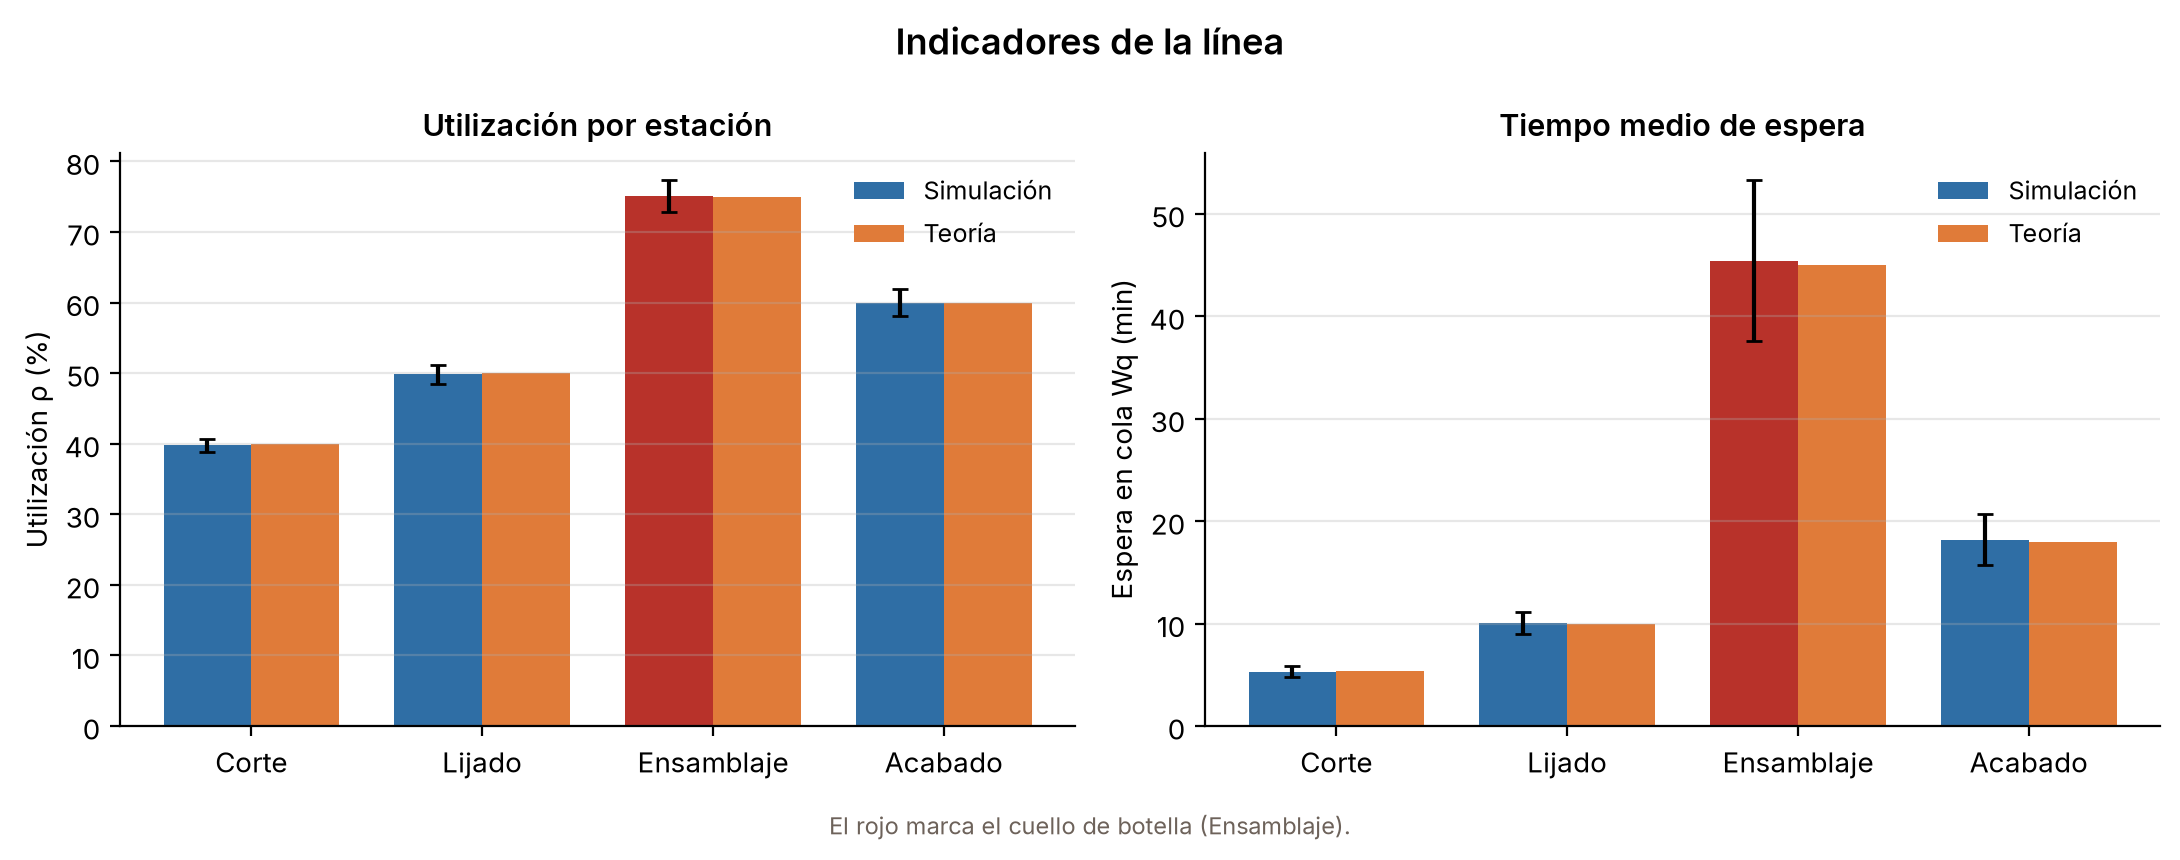
\includegraphics[width=\columnwidth]{base.png}
\caption{Utilización y espera por estación en E1: medias simuladas (con desviación estándar)
y referencias teóricas M/M/1.}
\label{fig:base}
\end{figure}

En el escenario base, ensamblaje presentó la menor capacidad nominal, con 4 muebles/h, y la
mayor utilización, del 75,10\,\%. También registró la mayor cola media, de 2,274 muebles, y
el mayor tiempo de espera, de 45,43 minutos. Estos resultados permitieron identificarla como
el cuello de botella inicial de la línea. Acabado presentó la segunda mayor utilización, con
un 59,99\,\%, y un tiempo de espera de 18,20 minutos (Fig.~\ref{fig:base}).

En las 900 horas de medición se terminaron, en promedio, 2\,698,43 $\pm$ 52,65 muebles por
réplica, equivalentes a una producción efectiva de 2,998 muebles/h. El tiempo total de flujo
fue de 123,96 $\pm$ 10,30 minutos por mueble. La comparación con el modelo M/M/1 mostró
diferencias reducidas en los indicadores de desempeño. Como se presenta en la Tabla
\ref{tab:errores}, el mayor error porcentual del escenario inicial fue del 1,26\,\%,
correspondiente a la longitud media de la cola de acabado.

\subsection{Resultados del objetivo específico 2}
Se comparó la línea inicial (E1) con dos escenarios de mejora que mantienen un único recurso
en ensamblaje. En E2, el tiempo medio de procesamiento de esta estación se redujo de 15 a 12
minutos, mientras que en E3 se redujo a 10 minutos. Los tres escenarios utilizaron la misma
tasa de llegadas, de 3 muebles/h, y 30 réplicas con 900 horas de medición por réplica.

\begin{table}[!t]
\caption{Comparación de capacidad e indicadores simulados en los tres escenarios (media
$\pm$ desviación estándar; $n = 30$)}
\label{tab:comparacion}
\centering
\scriptsize
\tablabase
\begin{tabular}{|L{2.5cm}|C{1.8cm}|C{1.8cm}|C{1.8cm}|}
\hline
\textbf{Indicador} & \textbf{E1 $\cdot$ Base} & \textbf{E2 $\cdot$ 12 min} &
\textbf{E3 $\cdot$ 10 min} \\ \hline
Capacidad de la línea (muebles/h) & 4,00 & 5,00 & 5,00 \\ \hline
Estación(es) de menor capacidad & Ensamblaje & Ensamblaje y acabado & Acabado \\ \hline
Utilización de ensamblaje (\%) & 75,10 $\pm$ 2,27 & 59,84 $\pm$ 1,92 & 49,72 $\pm$ 1,19 \\ \hline
Cola en ensamblaje $L_q$ (muebles) & 2,274 $\pm$ 0,418 & 0,865 $\pm$ 0,115 &
0,484 $\pm$ 0,046 \\ \hline
Espera en ensamblaje $W_q$ (min) & 45,43 $\pm$ 7,88 & 17,27 $\pm$ 2,09 & 9,71 $\pm$ 0,84 \\ \hline
Tiempo total de flujo (min) & 123,96 $\pm$ 10,30 & 92,25 $\pm$ 4,08 & 82,19 $\pm$ 2,78 \\ \hline
Muebles terminados por réplica & 2\,698,4 $\pm$ 52,7 & 2\,699,4 $\pm$ 56,9 &
2\,689,3 $\pm$ 40,6 \\ \hline
Producción efectiva (muebles/h) & 2,998 & 2,999 & 2,988 \\ \hline
\end{tabular}
\end{table}

Los resultados de la Tabla \ref{tab:comparacion} muestran que, en E2, reducir el tiempo de
ensamblaje de 15 a 12 minutos disminuyó la espera media de 45,43 a 17,27 minutos, lo que
representa una reducción del 61,99\,\%. De igual manera, la cola media pasó de 2,274 a 0,865
muebles, con una disminución aproximada del 61,97\,\%, mientras que la utilización de
ensamblaje se redujo del 75,10\,\% al 59,84\,\%.

En E3, al reducir el tiempo de ensamblaje a 10 minutos, la espera media llegó a 9,71
minutos, equivalente a una reducción del 78,62\,\% respecto a E1. La cola media disminuyó a
0,484 muebles, lo que representa una reducción aproximada del 78,72\,\%, y la utilización
alcanzó el 49,72\,\%. Por tanto, E3 presentó las mayores reducciones de cola y espera entre
los escenarios evaluados (Fig.~\ref{fig:escenarios}).

\begin{figure}[!t]
\centering
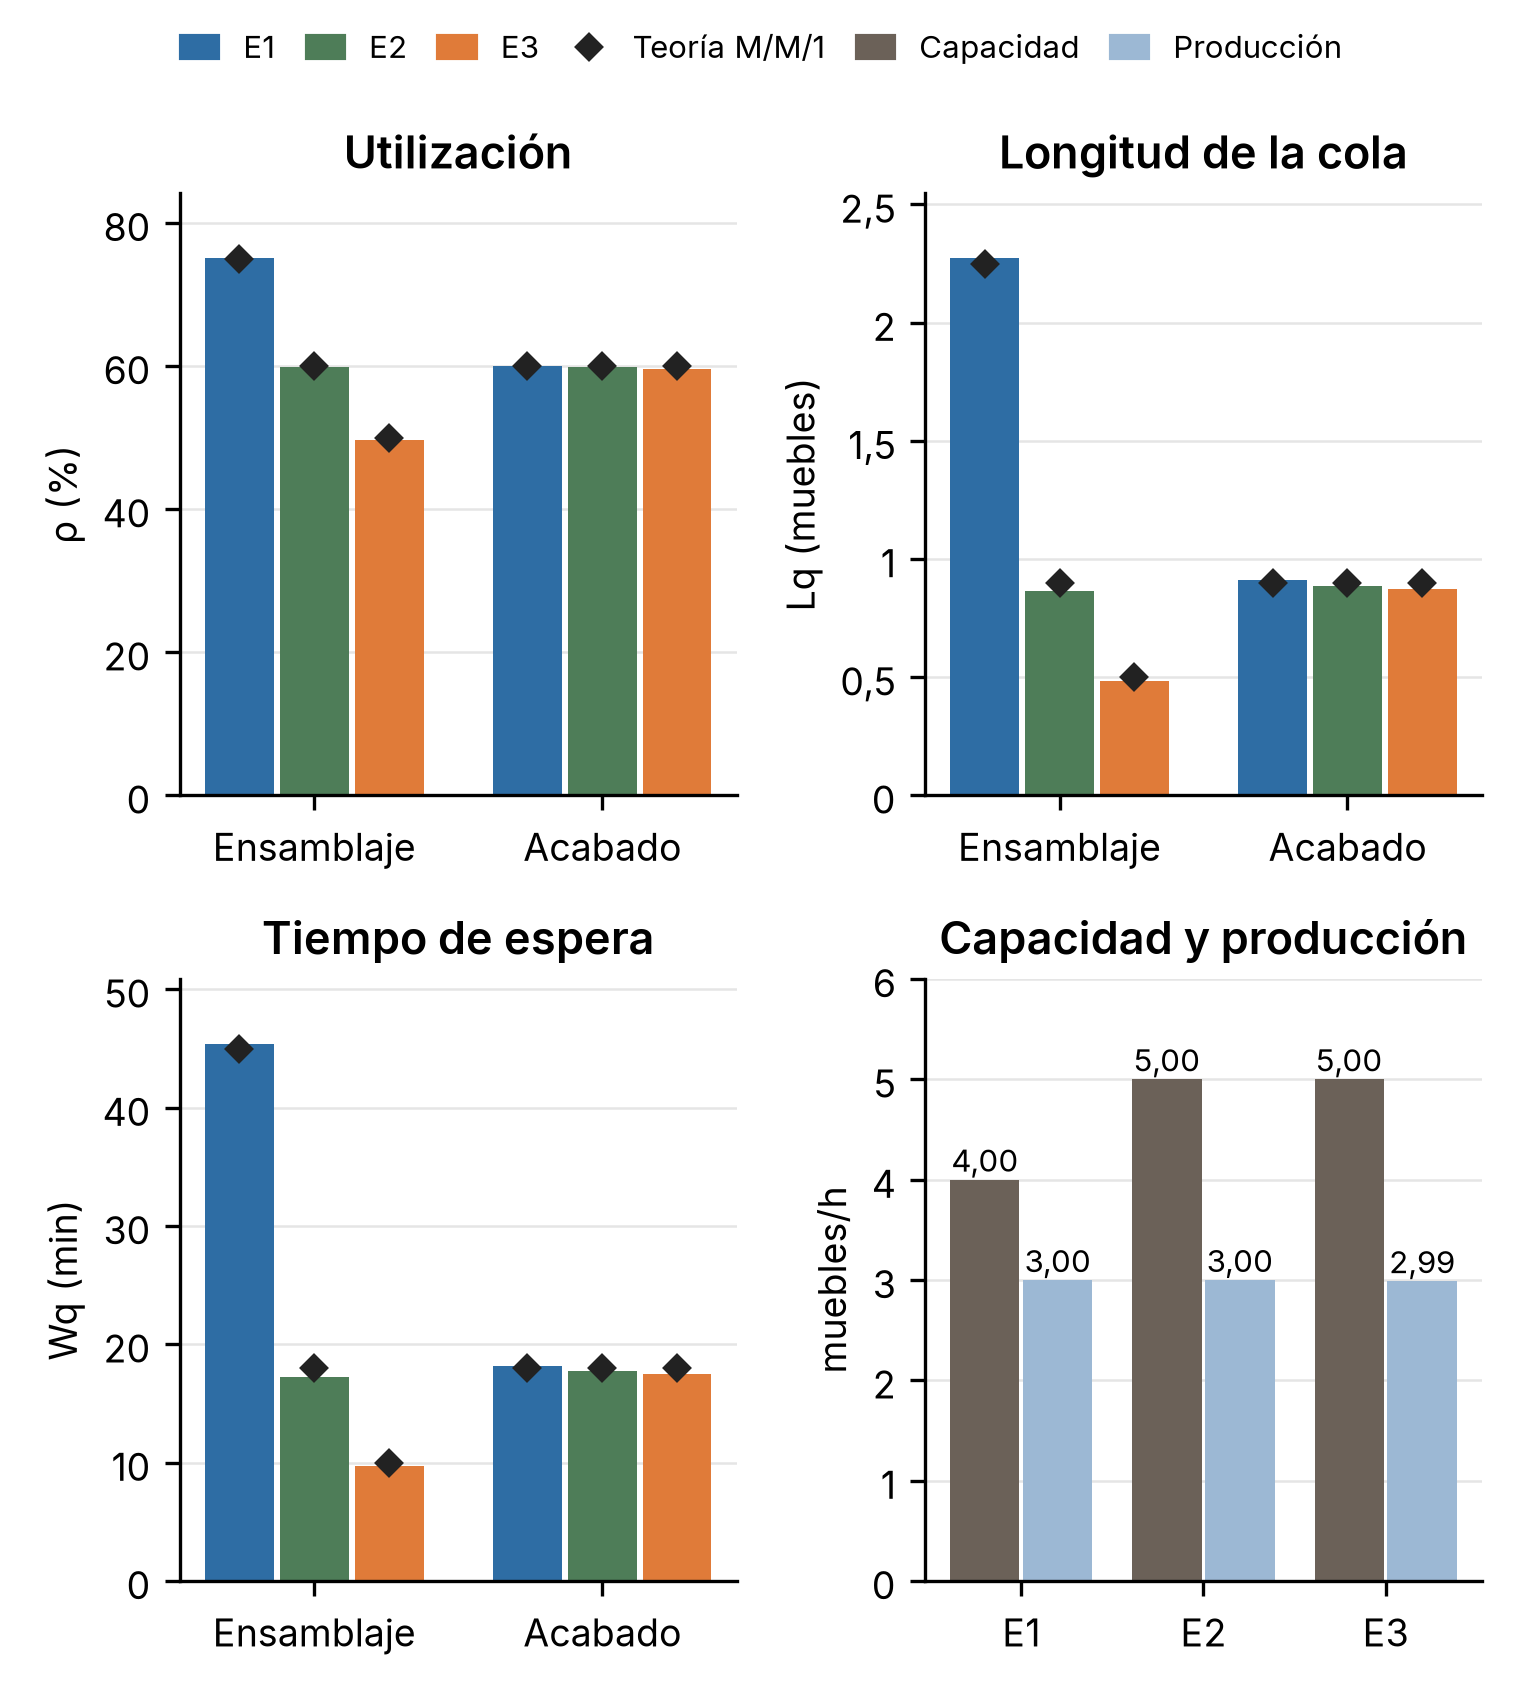
\includegraphics[width=\columnwidth]{escenarios-2x2.png}
\caption{Comparación de E1, E2 y E3 en las estaciones críticas (ensamblaje y acabado):
utilización, longitud de la cola y tiempo de espera simulados frente a la teoría M/M/1, y
capacidad de la línea frente a la producción simulada.}
\label{fig:escenarios}
\end{figure}

En cuanto a la capacidad máxima de producción, E2 y E3 alcanzaron 5 muebles/h, frente a los 4
muebles/h de E1, lo que representa un incremento del 25\,\%. En E2, ensamblaje y acabado
quedaron empatados en capacidad, con 5 muebles/h cada uno. En E3, acabado pasó a ser el cuello
de botella, ya que su capacidad permaneció en 5 muebles/h, mientras que ensamblaje alcanzó 6
muebles/h. Por ello, reducir aún más el tiempo de ensamblaje no incrementó la capacidad máxima
de la línea.

La producción efectiva se mantuvo cercana a los 3 muebles/h en los tres escenarios, debido a
que la tasa de llegadas utilizada en la simulación fue de 3 muebles/h. Esto significa que las
mejoras aumentaron la capacidad disponible de la línea, pero no la producción observada, que
permaneció limitada por la demanda simulada.

También se observó una reducción del tiempo total de flujo, que pasó de 123,96 minutos en E1
a 92,25 minutos en E2 y 82,19 minutos en E3. Estas diferencias representan disminuciones del
25,58\,\% y del 33,70\,\%, respectivamente, respecto al escenario inicial.

Para validar los resultados de la simulación frente al modelo M/M/1, se calcularon los
errores porcentuales de utilización ($\rho$), longitud media de cola ($L_q$) y tiempo medio de
espera ($W_q$) para cada escenario y estación. Los valores obtenidos se presentan en la Tabla
\ref{tab:errores}.

\begin{table}[!t]
\caption{Errores porcentuales entre la simulación y los valores teóricos por escenario y
estación}
\label{tab:errores}
\centering
\footnotesize
\tablabase
\begin{tabular}{|C{0.9cm}|L{1.9cm}|C{1.5cm}|C{1.5cm}|C{1.5cm}|}
\hline
\textbf{Esc.} & \textbf{Estación} & \textbf{Error $\boldsymbol{\rho}$ (\%)} &
\textbf{Error $\boldsymbol{L_q}$ (\%)} & \textbf{Error $\boldsymbol{W_q}$ (\%)} \\ \hline
E1 & Corte & 0,52 & 0,13 & 0,17 \\ \hline
E1 & Lijado & 0,36 & 0,18 & 0,13 \\ \hline
E1 & Ensamblaje & 0,14 & 1,06 & 0,94 \\ \hline
E1 & Acabado & 0,01 & 1,26 & 1,11 \\ \hline
E2 & Corte & 0,10 & 0,99 & 1,07 \\ \hline
E2 & Lijado & 0,13 & 0,37 & 0,31 \\ \hline
E2 & Ensamblaje & 0,27 & 3,92 & 4,07 \\ \hline
E2 & Acabado & 0,27 & 1,46 & 1,62 \\ \hline
E3 & Corte & 0,31 & 0,92 & 0,59 \\ \hline
E3 & Lijado & 0,92 & 2,05 & 1,86 \\ \hline
E3 & Ensamblaje & 0,56 & 3,18 & 2,88 \\ \hline
E3 & Acabado & 0,60 & 3,22 & 2,97 \\ \hline
\end{tabular}
\end{table}

Los errores porcentuales fueron reducidos en los tres escenarios. El error máximo de E1 fue
del 1,26\,\%, mientras que en E2 alcanzó el 4,07\,\% y en E3 llegó al 3,22\,\%. Estos
resultados muestran que las medidas simuladas se mantuvieron próximas a las predicciones del
modelo M/M/1, aunque las diferencias fueron mayores en algunos indicadores de los escenarios
de mejora.

En ensamblaje, los tiempos de espera teóricos fueron de 45,00, 18,00 y 10,00 minutos para
E1, E2 y E3, respectivamente. En la simulación se obtuvieron 45,43, 17,27 y 9,71 minutos, lo
que evidencia una correspondencia entre los valores simulados y teóricos.

Finalmente, mediante la Ley de Little se comprobó la relación entre la longitud media de las
colas y el tiempo de espera, obteniendo errores del 0,169\,\% en E1, 0,155\,\% en E2 y
0,134\,\% en E3. En conjunto, los resultados muestran que reducir el tiempo de ensamblaje
disminuyó las colas y las esperas, redujo el tiempo total de flujo y aumentó la capacidad
máxima de la línea del escenario inicial al segundo. Sin embargo, la capacidad permaneció en 5
muebles/h en E3 debido a que acabado se convirtió en el nuevo cuello de botella.

% ============================================================
\section{Discusión}
% ============================================================
En el escenario inicial, ensamblaje se identificó como el cuello de botella debido a su menor
capacidad y mayor tiempo de espera. Este comportamiento coincide con los estudios de Bambura
\textit{et al.} \cite{bambura2020} y Velumani y Tang \cite{velumani2017}, quienes utilizaron
simulación para identificar restricciones en líneas de producción. Asimismo, Wu y McGinnis
\cite{wu2012} explican la relación entre la utilización de los recursos y el aumento de las
esperas. En este caso, las llegadas y los tiempos de procesamiento aleatorios provocaron
acumulaciones en ensamblaje, aun cuando su utilización no alcanzaba el 100\,\%.

Las mejoras aplicadas redujeron las esperas en ensamblaje un 61,99\,\% en E2 y un 78,62\,\%
en E3. Estos resultados son consistentes con Li \textit{et al.} \cite{li2020}, quienes
estudiaron cómo aumentar la capacidad de una estación crítica mejora el desempeño de una
línea. Sin embargo, mientras dicho estudio evaluó la incorporación de máquinas, aquí se
disminuyó el tiempo de procesamiento. En E2, ensamblaje y acabado quedaron con la misma
capacidad, mientras que en E3 acabado pasó a ser la estación limitante. Esto demuestra que
mejorar una operación puede trasladar el cuello de botella hacia otra etapa.

Aunque ambas mejoras aumentaron un 25\,\% la capacidad nominal de la línea, la producción
efectiva permaneció cercana a tres muebles por hora, debido a que la tasa de llegadas se
mantuvo constante. En cambio, disminuyeron las colas y el tiempo total de flujo. Este
comportamiento se relaciona con los trabajos de Nouri y Abdul-Nour \cite{nouri2019} y Mat
Rani \textit{et al.} \cite{matrani2026}, quienes analizaron cómo las modificaciones operativas
pueden mejorar el desempeño de sistemas de fabricación de muebles, aunque bajo condiciones y
configuraciones diferentes.

Por otra parte, los errores porcentuales entre la simulación y los valores teóricos no
superaron el 4,07\,\%, lo que muestra una correspondencia cercana con los modelos de teoría de
colas descritos por Govil y Fu \cite{govil1999} y Gross \textit{et al.} \cite{gross2008}. Las
diferencias pueden relacionarse con la variabilidad aleatoria y la duración finita de los
experimentos. Esta concordancia respalda la consistencia del modelo bajo los supuestos
establecidos, pero no constituye una validación frente a una fábrica real.

Finalmente, el uso de Python permitió comparar alternativas sin modificar físicamente una
línea de producción, una ventaja de la simulación señalada por Negahban y Smith
\cite{negahban2014} y Mourtzis \cite{mourtzis2020}. No obstante, el modelo utiliza parámetros
hipotéticos y excluye fallas, defectos y costos operativos, por lo que sus resultados no
pueden aplicarse directamente a una fábrica. Su principal aporte es integrar la
identificación de cuellos de botella, la evaluación de mejoras y la comparación con la teoría
de colas mediante una herramienta gratuita y reproducible.

% ============================================================
\section{Conclusiones}
% ============================================================
El modelo de simulación desarrollado representó el comportamiento de la línea de producción
de muebles con resultados cercanos a los valores teóricos (objetivo específico 1). En la
línea base, el error porcentual frente al modelo M/M/1 fue menor al 0,6\,\% en la utilización
y no superó el 1,3\,\% en las colas y los tiempos de espera, y la Ley de Little se cumplió
con un error del 0,169\,\%. Esto confirma que el modelo es consistente con la teoría y
permite evaluar cambios operativos bajo las condiciones simuladas.

La estación de ensamblaje constituye el cuello de botella del sistema, lo que corrobora el
análisis de capacidades (objetivo específico 2). Esta estación alcanzó una utilización del
75,1\,\% y el mayor tiempo de espera, 45,4 minutos, que representa aproximadamente el
37\,\% del tiempo total de flujo de cada mueble.

Reducir el tiempo de procesamiento de la estación crítica alivia la congestión de la línea
(objetivo específico 2). Acortar el ensamblaje de 15 a 12 y 10 minutos redujo su espera en un
61,99\,\% y un 78,62\,\%, y elevó la capacidad de la línea de 4 a 5 muebles por hora
(25\,\%). Sin embargo, en E3 el cuello de botella se trasladó a acabado, y la producción
efectiva se mantuvo cerca de 3 muebles por hora, porque la limita la tasa de llegadas y no la
capacidad.

% ============================================================
\section{Recomendaciones}
% ============================================================
Modificar el modelo en Python (SimPy) para incorporar fallas de maquinaria, tiempos de
mantenimiento, defectos de calidad y reprocesos, ya que el modelo actual asume condiciones
ideales donde las piezas y la madera siempre están disponibles y sin defectos.

El experimento se ejecuta como un sistema continuo durante 1\,000 horas para lograr un estado
estable. Se recomienda adaptar el código en Python para reflejar turnos de trabajo reales
(por ejemplo, jornadas de 8 horas con paradas por almuerzo y tiempos de preparación inicial),
lo que daría una visión más exacta de las colas que quedan pendientes al final del día.

Evaluar escenarios con una tasa de llegadas mayor a 3 muebles por hora y mejoras combinadas
en ensamblaje y acabado, ya que con la demanda actual el aumento de capacidad no se reflejó
en la producción efectiva y, en E3, acabado pasó a limitar la línea.

% ============================================================
% Referencias (numeradas por orden de cita) y bibliografía
% ============================================================
\bibliographystyle{IEEEtran}
\bibliography{referencias}

\section*{Bibliografía}
{\footnotesize
Documentación técnica consultada para la implementación y no citada en el texto:

\begin{list}{}{\setlength{\leftmargin}{0.65cm}\setlength{\itemindent}{0pt}%
\setlength{\itemsep}{2pt}\setlength{\topsep}{2pt}\setlength{\parsep}{0pt}}
\item Team SimPy, ``SimPy: Discrete event simulation for Python'', versión 4.1. [En línea].
Disponible: \url{https://simpy.readthedocs.io/}
\item NumPy Developers, ``NumPy documentation'', versión 2.5. [En línea]. Disponible:
\url{https://numpy.org/doc/}
\item The pandas development team, ``pandas documentation'', versión 3.0. [En línea].
Disponible: \url{https://pandas.pydata.org/docs/}
\item The Matplotlib development team, ``Matplotlib documentation'', versión 3.11. [En
línea]. Disponible: \url{https://matplotlib.org/stable/}
\end{list}
}

% ============================================================
\section*{Declaratoria de uso de inteligencia artificial}
% ============================================================
\noindent\textbf{Herramienta utilizada 1:} ChatGPT.

\noindent\textbf{Forma de uso:} se utilizó ChatGPT como apoyo para analizar los resultados
obtenidos en las simulaciones de la línea de producción. Para ello, se compartieron tablas y
gráficas generadas durante los experimentos, con el fin de interpretar los datos, comparar los
escenarios e identificar los principales resultados relacionados con la utilización de las
estaciones, las colas, los tiempos de espera y la capacidad de producción.

\noindent\textbf{Prompt utilizado:} \textit{``Te envío las gráficas y tablas obtenidas de las
simulaciones de la línea de producción de sillas. Ayúdame a interpretar los resultados,
comparar los escenarios y explicar qué muestran los datos sobre los tiempos de espera, las
colas, la utilización de las estaciones y la capacidad de producción.''}

\medskip
\noindent\textbf{Herramienta utilizada 2:} NotebookLM.

\noindent\textbf{Forma de uso:} se utilizó NotebookLM para consultar los artículos científicos
seleccionados, obtener información relevante sobre su contenido y comprender sus aportes al
tema de investigación. También se empleó para recopilar y organizar la información
bibliográfica necesaria para elaborar las referencias en formato IEEE.

\noindent\textbf{Prompt utilizado:} \textit{``Analiza los artículos científicos
proporcionados y extrae sus principales aportes, los objetivos de cada investigación y la
información relevante para contextualizar nuestro trabajo. Además, identifica los datos
bibliográficos necesarios para elaborar las referencias en formato IEEE, utilizando
únicamente la información disponible en los documentos.''}

\medskip
\noindent\textbf{Herramienta utilizada 3:} Claude (Anthropic), modelos Claude Opus 5.5 y
Claude Sonnet 5.5, mediante los asistentes de programación Claude Code y Pi.

\noindent\textbf{Forma de uso:} se utilizaron estos modelos como asistentes de programación
para generar y revisar el código de la simulación en Python (modelo de eventos discretos con
SimPy, cálculo teórico M/M/1, animación y panel de parámetros), escribir pruebas
automáticas, detectar y corregir errores, y redactar la documentación técnica del proyecto
(README). Los integrantes definieron el modelo, los parámetros y los escenarios, revisaron
los cambios realizados y verificaron los resultados mediante su comparación con la teoría de
colas. Los prompts utilizados se presentan en la Tabla \ref{tab:b1} del Anexo B.

\medskip
\noindent\textit{Nota:} los prompts de la Tabla \ref{tab:b1} se transcriben con la ortografía
corregida, sin modificar su sentido. El prompt de la herramienta 1 se conserva textualmente.
El uso de estas herramientas no exime a los integrantes de la responsabilidad sobre el
contenido, los resultados, las referencias y las conclusiones del trabajo, que fueron
verificados por el grupo.

% ============================================================
% Anexos (una columna: tablas de ancho completo)
% ============================================================
\onecolumn
\section*{Anexos}

\noindent\textit{Anexo A. Trabajos relacionados}

\setcounter{table}{0}
\renewcommand{\thetable}{A\arabic{table}}
\renewcommand{\arraystretch}{1.15}
\setlength{\tabcolsep}{3pt}
{\scriptsize
\begin{longtable}{|L{4.2cm}|C{1.0cm}|L{6.3cm}|L{5.4cm}|}
\caption{Trabajos relacionados y aportes al proyecto}\label{tab:a1}\\
\hline
\textbf{Artículo} & \textbf{Ref.} & \textbf{Qué hicieron} &
\textbf{Qué aporta a este trabajo} \\ \hline
\endfirsthead
\hline
\textbf{Artículo} & \textbf{Ref.} & \textbf{Qué hicieron} &
\textbf{Qué aporta a este trabajo} \\ \hline
\endhead
Optimization via computer simulation of a mixed assembly line of wooden furniture---A case
study & \cite{nouri2019} & Estudio de caso de una línea de ensamblaje y acabado donde se
fabrican varios tipos de muebles de madera. Con el programa Arena y diseño de experimentos,
vieron cómo influyen la variedad de productos, el orden en que se programan los trabajos y
los colores. & Es un antecedente directo en muebles de madera: muestra cómo el orden de los
trabajos y la mezcla de productos cambian los tiempos y las colas. \\ \hline
Optimal worker allocation of wooden furniture manufacturing system using simulation modeling
and data envelopment analysis & \cite{matrani2026} & Estudiaron cuántos trabajadores asignar
en una línea que fabrica mesas de madera con 9 procesos. Combinaron simulación en Arena con
el método DEA (análisis envolvente de datos), que compara qué tan eficiente es cada
alternativa. & Sirve de ejemplo para modelar los procesos de una fábrica de madera y muestra
que repartir mejor los recursos reduce las esperas entre estaciones. \\ \hline
Utilization of computer simulation for optimization of furniture production system &
\cite{bambura2020} & Simularon en Plant Simulation la producción de una cajonera y
encontraron que el lijado y el ensamblaje eran los cuellos de botella. & Es un ejemplo
práctico de cómo hallar cuellos de botella en muebles de madera, y muestra que añadir
máquinas ayuda a equilibrar la línea. \\ \hline
Operations status and bottleneck analysis and improvement of a batch process manufacturing
line using discrete event simulation & \cite{velumani2017} & Con simulación, analizaron cómo
funcionaba una línea que produce por lotes: dónde estaban los cuellos de botella y cuántas
piezas se acumulaban en proceso. & Da indicadores para medir las esperas, la acumulación de
piezas y los bloqueos entre etapas de una línea en serie. \\ \hline
Bottleneck identification and alleviation in a blocked serial production line with discrete
event simulation: A case study & \cite{li2020} & Compararon cinco métodos para encontrar el
cuello de botella en una línea de etapas en serie donde unas etapas pueden bloquear a otras.
Usaron Plant Simulation y probaron qué pasa al aumentar la capacidad de la etapa crítica. &
Ofrece formas de comparar métodos para hallar el cuello de botella y muestra que añadir
máquinas en esa etapa mejora la línea, pero cada vez menos. \\ \hline
Simulation for manufacturing system design and operation: Literature review and analysis &
\cite{negahban2014} & Revisaron casi 300 trabajos sobre simulación de eventos discretos en el
diseño y la operación de fábricas, y notaron que cada vez se usa más para decidir sobre la
operación diaria. & Es la base para justificar el uso de la simulación de eventos discretos y
para encontrar problemas en líneas de producción. \\ \hline
Simulation in the design and operation of manufacturing systems: State of the art and new
trends & \cite{mourtzis2020} & Cuenta cómo ha cambiado la simulación en la industria durante
unos sesenta años y cómo las tecnologías digitales ayudan a probar alternativas antes de
aplicarlas en la planta. & Justifica hacer un modelo en Python para probar cambios en la
producción de muebles sin gastar dinero ni detener la planta. \\ \hline
Queueing theory in manufacturing: A survey & \cite{govil1999} & Revisaron los modelos de
teoría de colas usados en manufactura. Los dividen en los que miden el desempeño de un
sistema y los que sirven para diseñarlo y controlarlo. & Da las ecuaciones para calcular
esperas y utilización, que aquí se usan para comprobar los resultados de la simulación. \\
\hline
Performance evaluation for general queueing networks in manufacturing systems:
Characterizing the trade-off between queue time and utilization & \cite{wu2012} & Plantean
cómo calcular el cambio del tiempo de espera según qué tan ocupado está un recurso, en redes
de colas complejas. & Explica por qué un recurso muy ocupado genera esperas mucho mayores y
ayuda a reconocer cuellos de botella con cálculos. \\ \hline
\end{longtable}
}

\bigskip
\noindent\textit{Anexo B. Prompts utilizados para el desarrollo del código}

\setcounter{table}{0}
\renewcommand{\thetable}{B\arabic{table}}
{\scriptsize
\begin{longtable}{|C{1.0cm}|C{2.0cm}|L{7.8cm}|L{6.1cm}|}
\caption{Prompts utilizados con Claude para el desarrollo del código}\label{tab:b1}\\
\hline
\textbf{N.º} & \textbf{Fecha} & \textbf{Prompt utilizado} & \textbf{Uso de la IA} \\ \hline
\endfirsthead
\hline
\textbf{N.º} & \textbf{Fecha} & \textbf{Prompt utilizado} & \textbf{Uso de la IA} \\ \hline
\endhead
1 & 21/10/2026 & \textit{``Más bien adapta mi parte a lo que ya existe del documento sin
cambiar el plan.''} & Ajustar la tarea de simulación al plan del grupo (parámetros,
réplicas y escenarios). \\ \hline
2 & 21/10/2026 & \textit{``Dale, programa, coloca resultados y actualiza el
documento.''} & Generar el modelo de eventos discretos en SimPy, la teoría M/M/1, las
pruebas y los resultados de la línea base. \\ \hline
3 & 21/10/2026 & \textit{``Hagamos que la simulación tenga un nivel superior y hazla
realista usando HTML y recursos que refuercen el proyecto y el aprendizaje.''} & Prototipo
de simulador web, descartado posteriormente (prompt 6). \\ \hline
4 & 27/10/2026 & \textit{``Dale con todos los pendientes.'' / ``Soluciona los dos
menores.''} & Corregir los errores detectados en la revisión del código. \\ \hline
5 & 27/10/2026 & \textit{``¿Se indica bien en el README cómo levantar la simulación y todo
claro? ¿Comentaste el código para entenderlo, hiciste lo más simple, no hay datos quemados y
hay cómo cambiar escenarios?''} & Revisar la claridad del código, los comentarios, los
valores fijos y la configuración de escenarios. \\ \hline
6 & 27/10/2026 & \textit{``No lo hagamos con web, hagámoslo con puro Python. Y cubre las
falencias.''} & Dejar la implementación solo en Python y agregar los escenarios E2 y E3
mediante archivos JSON. \\ \hline
7 & 27/10/2026 & \textit{``Haz una simulación bien visual y fácil de entender, pero como
si fuera el ejemplo real; no quiero círculos imaginarios.''} & Generar la animación del
taller con Matplotlib. \\ \hline
8 & 27/10/2026 & \textit{``Se rompe el texto, cambia de tipo de letra; mejora el tema de la
gráfica de abajo y asegúrate de que todo esté claro.''} & Corregir la legibilidad de la
animación (fuente y gráfico inferior). \\ \hline
9 & 28/10/2026 & \textit{``Hay un último push de un compañero, revísalo.'' / ``Sí, corrige
esos dos puntos.''} & Revisar la reestructuración del código en modelo, vista y controlador
(MVC) y corregir la validación de valores NaN e infinitos. \\ \hline
10 & 28/10/2026 & \textit{``¿Ya funciona lo de cambiar valores? ¿Anda la simulación en
cualquier caso planteado?''} & Probar la simulación con valores arbitrarios, incluido un
caso saturado ($\rho \geq 1$). \\ \hline
11 & 28/10/2026 & \textit{``El docente siempre pide cambiar los valores a los que él desee;
hay que agregar esa parte en lo visual, y en el código tiene que estar bien claro dónde
cambiarlos.''} & Generar el panel de parámetros (panel.py) y documentar dónde cambiar cada
valor. \\ \hline
12 & 28/10/2026 & \textit{``Revisa los últimos avances del git y mira si ya cumple.'' /
``¿Y en cuanto al código?''} & Verificar las pruebas, la coincidencia de los resultados del
informe con los de la simulación y la actualización de los README. \\ \hline
13 & 28/10/2026 & \textit{``Ojo, que el proyecto ahora es de muebles; míralo y contrástalo
con el documento y el código: todo debe ser de muebles.''} & Cambiar la terminología de
``sillas'' a ``muebles'' en el código, los CSV y los gráficos, sin alterar los
resultados. \\ \hline
\end{longtable}
}

\bigskip
\noindent\textit{Anexo C. Repositorio del código}

\vspace{2pt}
{\small
\noindent El código, los escenarios, las pruebas y los resultados están en el repositorio
público \url{https://github.com/AlejandroTatum/simulacion-linea-muebles} (rama main): el
código y los escenarios E1--E3 en \texttt{03-simulacion/}, los resultados en
\texttt{04-experimentos/} y las fuentes del informe en \texttt{05-informe/}. El README explica
la instalación; \texttt{main.py} ejecuta E1--E3 y \texttt{panel.py} permite cambiar los
parámetros y simular en vivo.}

\end{document}
